\documentclass{article}
\usepackage[headheight=40pt, textheight=560pt]{geometry}
\usepackage{paralist}
\usepackage{scalerel,amssymb}
\usepackage{amsmath}
\usepackage{colortbl}
\usepackage{array}
\usepackage{multirow}
\usepackage{blindtext}
\usepackage{reledmac}
\usepackage{changepage}

\usepackage{pgfplots}
\usepackage{tikz}
\usetikzlibrary{positioning}
\usetikzlibrary{shapes.geometric, arrows}
\usetikzlibrary{decorations.pathreplacing}
\tikzstyle{arrow} = [thick,->,>=stealth]

\usepackage{graphicx}
\usepackage{stix}

\newcommand{\tableflip}{$($\rotatebox{45}{$\smile$}$^{\circ}\smwhtsquare^{\circ})\rotatebox{45}{$\smile$}\mkern-6mu\frown$\raisebox{0.5ex}{$\bot$}$\mkern-3.5mu-\mkern-3.5mu$\raisebox{0.5ex}{$\bot$}}

\usepackage{stackengine}
\def\apeqA{\SavedStyle\sim}
\def\apeq{\setstackgap{L}{\dimexpr.5pt+1.5\LMpt}\ensurestackMath{%
  \ThisStyle{\mathrel{\Centerstack{{\apeqA} {\apeqA} {\apeqA}}}}}}

\usepackage{fancyhdr}
\fancyhead[L]{
	\begin{tabular}{ll}
		\begin{tabular}{l}
			\includegraphics[scale=0.13]{distributed}
		\end{tabular}	
		&
		\begin{tabular}{l}
			\LARGE \textbf{Distributed Algorithms} \\
			\Large \textsc{Lectures}
		\end{tabular}
	\end{tabular}
}
\fancyhead[R]{
	\begin{tabular}{r}
		16-124-836 \\
		Marcel \textsc{Zauder}
	\end{tabular}
}
\renewcommand{\headrulewidth}{0.4pt}
\fancyfoot[C]{\thepage}
\renewcommand{\footrulewidth}{0.4pt}

\usepackage{hyperref}

\begin{document}
	\pagestyle{fancy}
	\section{Introduction - February 19, 2020}
	\begin{adjustwidth}{2em}{2em}
		\subsection{Defining Dependable Systems}
		\begin{adjustwidth}{2em}{2em}
			\textsc{Quotes:}
			\begin{adjustwidth}{2em}{}
				\textit{A distributed system is a system where a computer of which you did not know it exists can prevent you from getiing your job done.} - Leslie \textsc{Lamport}
			\end{adjustwidth}
			\vspace{0.2cm}
			\begin{adjustwidth}{2em}{}
				\textit{There is perhaps a market for maybe five computers in the world.} - TJ \textsc{Watson}
			\end{adjustwidth}
			\hfill \\
			\textsc{Fault} $\rightarrow$ \textsc{Error} $\rightarrow$ \textsc{Failure}
			\begin{compactenum}[-]
				\item Train delayed because of tree has fallen on the tracks
				\item Travelers reach destination too late
				\item Alice misses her exam
			\end{compactenum}
			\vspace{0.2cm}
			\begin{tabular}{|l|lll|}
				\hline
				& \underline{\textsc{Fault}} & \underline{\textsc{Error}} & \underline{\textsc{Failure}} \\
				\hline
				Train: & Tree fallen & no train & delay for passengers \\
				Journey: & Train delay & delay & reached destination 2h after intention \\
				Exam: & arrival 2h late & missed time-slot & repeat exam \\
				\hline
			\end{tabular}
			\hfill \\
			\underline{\textsc{Fault:}} cause of failure \\
			\underline{\textsc{Error:}} internal state of system, not according to specification \\
			\underline{\textsc{Failure:}} observable deviation of specification
			\hfill \\ \\
			\underline{\textsc{Fault} examples:}
			\begin{compactenum}[-]
				\item timing
				\item cables
				\item power supply
				\item messages lost
				\item data loss (solved with RAIDs)
			\end{compactenum}
			\subsubsection{\underline{How to make systems tolerate faults}}
			\begin{adjustwidth}{2em}{}
				\begin{compactenum}[-]
					\item \textsc{Prevention}
					\item \textsc{Tolerance}
					\begin{compactenum}[\textbullet]
						\item Replication/Redundancy
						\item Recovery
					\end{compactenum}
					\item \textsc{Removal}
					\item \textsc{Forecasting/Prediction}
				\end{compactenum}
			\end{adjustwidth}
			\hfill \\
			\textsc{Safety} $\neq$ \textsc{Security} \\
			\textsc{Safety} is connected to loss of live/material due to accidents \\
			\textsc{Security} is connected to malicious intent
			\subsubsection{Defining distributed computation}
			\begin{adjustwidth}{2em}{}
				Processes $\Pi = \{ p,q,r,s \ldots \}$ \\
				$\mid \Pi \mid = N$
				
				\begin{adjustwidth}{1em}{}
					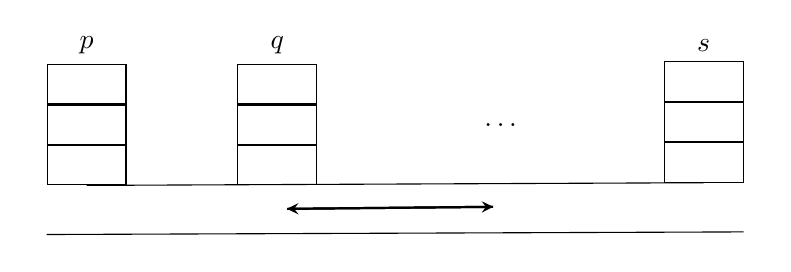
\begin{tikzpicture}
						\coordinate (start);
							
						%Nodes
						\node [right=of start] (p) {$p$};
						\node (rect) [draw,thin,minimum width=1cm,minimum height=0.5cm, below=0cm of p] (1stp) {};
						\node (rect) [draw,thin,minimum width=1cm,minimum height=0.5cm, below=0cm of 1stp] (2ndp) {};
						\node (rect) [draw,thin,minimum width=1cm,minimum height=0.5cm, below=0cm of 2ndp] (3rdp) {};
						
						\node [right=2cm of p] (q) {$q$};
						\node (rect) [draw,thin,minimum width=1cm,minimum height=0.5cm, below=0cm of q] (1stq) {};
						\node (rect) [draw,thin,minimum width=1cm,minimum height=0.5cm, below=0cm of 1stq] (2ndq) {};
						\node (rect) [draw,thin,minimum width=1cm,minimum height=0.5cm, below=0cm of 2ndq] (3rdq) {};
						
						\node [right=2cm of 2ndq] (ldots) {\ldots};
						
						\node [right=5cm of q] (s) {$s$};
						\node (rect) [draw,thin,minimum width=1cm,minimum height=0.5cm, below=0cm of s] (1sts) {};
						\node (rect) [draw,thin,minimum width=1cm,minimum height=0.5cm, below=0cm of 1sts] (2nds) {};
						\node (rect) [draw,thin,minimum width=1cm,minimum height=0.5cm, below=0cm of 2nds] (3rds) {};
						
						\node [below left=0.5cm and 0cm of 3rdp] (pbelow) {};	
						\node [below right=0.5cm and 0cm of 3rds] (sbelow) {};	
						\node [below =0.175cm of 3rdq] (qbelow) {};	
						\node [below =0.775cm of ldots] (ldotsbelow) {};	
						
						%Lines
						\draw (3rdp.south) -- (3rds.south);
						\draw (pbelow) -- (sbelow);
						\draw[arrow] (qbelow) -- (ldotsbelow);
						\draw[arrow] (ldotsbelow) -- (qbelow);
							
						%Lines
						%\draw[arrow] (start) -- node[ anchor=south ]{$m$} (Enc.west);
						%\draw[arrow] (Enc.east) -- node[ anchor=south ]{$c$} (Dec.west);
						%\draw[arrow] (Enc.east) -| (Eve.north);
						%\draw[arrow] (Dec.east) -- node[ anchor=south ]{$m'$} (stop.west);
							
					\end{tikzpicture}
				\end{adjustwidth}
				\hfill \\
				\underline{\textsc{Components}} \\
				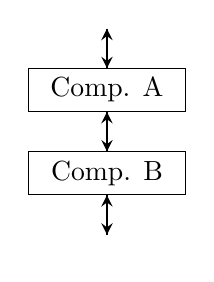
\begin{tikzpicture}					
					\coordinate (start);
					
					%Nodes
					\node (rect) [draw,thin,minimum width=2cm,minimum height=0.5cm, below=0.5cm of start] (CompA) {Comp. A};
					\node (rect) [draw,thin,minimum width=2cm,minimum height=0.5cm, below=0.5cm of CompA] (CompB) {Comp. B};
					\node [below=0.5cm of CompB] (stop) {};
					
					%Lines
					\draw[arrow] (start) -- (CompA.north);
					\draw[arrow] (CompA.north) -- (start);
					\draw[arrow] (CompA.south) -- (CompB.north);
					\draw[arrow] (CompB.north) -- (CompA.south);
					\draw[arrow] (stop) -- (CompB.south);
					\draw[arrow] (CompB.south) -- (stop);
				\end{tikzpicture}
				\hfill \\
				\textsc{Events} for Component $c$:
				\[
					\langle c, event \mid param_1 , param_2 \ldots \rangle
				\]
				\underline{upon} $\langle c, ev_1 \mid param_1 \rangle$ \underline{do}
				\begin{adjustwidth}{1em}{}
					do something \\
					\underline{trigger} $\langle \textit{b, domore} \mid p \rangle$
				\end{adjustwidth}
				\hfill \\
				\underline{upon} $\langle \textit{b, domore} \mid p \rangle$ \underline{do}
			\end{adjustwidth}
			\subsubsection{Layered modules}
			\begin{adjustwidth}{2em}{}
				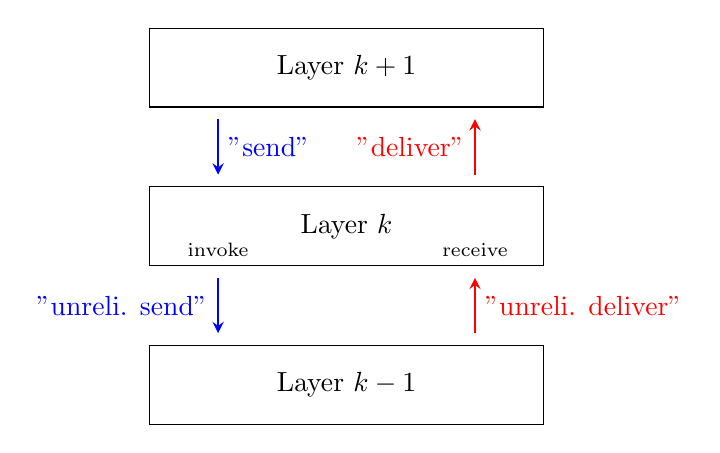
\begin{tikzpicture}
					\coordinate (start);
					
					%Nodes
					\node (rect) [draw,thin,minimum width=5cm,minimum height=1cm] (Layerk+1) {Layer $k+1$};
					\node (rect) [draw,thin,minimum width=5cm,minimum height=1cm, below=1cm of Layerk+1] (Layerk) {Layer $k$};
					\node (rect) [draw,thin,minimum width=5cm,minimum height=1cm, below=1cm of Layerk] (Layerk-1) {Layer $k-1$};
					
					\node [below left = -0.1cm and -1cm of Layerk+1] (sendOut) {};
					\node [below right = -0.1cm and -1cm of Layerk+1] (deliverIn) {};
					\node [above left = -0.1cm and -1cm of Layerk] (sendIn) {};
					\node [above right = -0.1cm and -1cm of Layerk] (deliverOut) {};
					\node [below left = -0.1cm and -1cm of Layerk] (unSendOut) {};
					\node [below right = -0.1cm and -1cm of Layerk] (unDeliverIn) {};
					\node [above left = -0.1cm and -1cm of Layerk-1] (unSendIn) {};
					\node [above right = -0.1cm and -1cm of Layerk-1] (unDeliverOut) {};
					
					\node [above=-0.1cm of unSendOut] (invoke) {\scriptsize invoke};
					\node [above=-0.1cm of unDeliverIn] (receive) {\scriptsize receive};
					
					%Lines
					\draw[blue, arrow] (sendOut) -- node[ anchor=west ]{"send"} (sendIn);
					\draw[red, arrow] (deliverOut) -- node[ anchor=east ]{"deliver"} (deliverIn);
					\draw[blue, arrow] (unSendOut) -- node[ anchor=east ]{"unreli. send"} (unSendIn);
					\draw[red, arrow] (unDeliverOut) -- node[ anchor=west ]{"unreli. deliver"} (unDeliverIn);
				\end{tikzpicture}
				\hfill \\
				Events either travel:
				\begin{compactenum}[-]
					\item upwards (red): indication
					\item downwards (blue): request
				\end{compactenum}
				\vspace{0.3cm}
				Events on a given layer may be:
				\begin{compactenum}[-]
					\item input events (IN)
					\item output events (OUT)
				\end{compactenum}
			\end{adjustwidth}
			\subsubsection{Module Jobhandler}
			\begin{adjustwidth}{2em}{}
				\underline{Events:}
				\begin{adjustwidth}{1em}{}
					Request: $\langle \textit{jh, handle} \mid \textit{job} \rangle$ \\
					Indication: $\langle \textit{jh, confirm} \mid \textit{job} \rangle$
				\end{adjustwidth}
				\underline{Properties:}
				\begin{adjustwidth}{1em}{}
					Every job submitted for handling is eventually confirmed.
				\end{adjustwidth}
				\hfill \\
				\underline{Implementation (synchronized)} \textsc{JobHandler} \\
				\underline{State}
				\begin{adjustwidth}{1em}{}
					\ldots
				\end{adjustwidth}
				\underline{upon} $\langle \textit{jh, handle} \mid \textit{job} \rangle$ \underline{do}
				\begin{adjustwidth}{1em}{}
					"process job" \\
					\underline{trigger} $\langle \textit{jh, confirm} \mid \textit{job} \rangle$
				\end{adjustwidth}
				\vspace{0.2cm}
				\underline{upon} \ldots \\
				\underline{upon} \ldots \\ \\
				\underline{Implementation (asynchronized)} \textsc{JobHandler} \\
				\underline{State}
				\begin{adjustwidth}{1em}{}
					\textit{buf} $\leftarrow \emptyset$
				\end{adjustwidth}
				\underline{upon} $\langle \textit{jh, handle} \mid \textit{job} \rangle$ \underline{do}
				\begin{adjustwidth}{1em}{}
					\textit{buf} $\leftarrow$ \textit{buf} $\cup \{ \textit{job} \}$ \\
					\underline{trigger} $\langle \textit{jh, confirm} \mid \textit{job} \rangle$
				\end{adjustwidth}
				\vspace{0.2cm}
				\underline{upon} \textit{buf} $\neq \emptyset$ \underline{do}
				\begin{adjustwidth}{1em}{}
					\textit{job} $\leftarrow$ some element of \textit{buf} \\
					"process job" \\
					\textit{buf} $\leftarrow$ \textit{buf} $\setminus \{ \textit{job} \}$
				\end{adjustwidth}
			\end{adjustwidth}
		\end{adjustwidth}
		\subsection{Concurrency and Replication in Distributed Systems}
		\begin{adjustwidth}{2em}{2em}
		\end{adjustwidth}
	\end{adjustwidth}
	
	\newpage
	
	\section{Models and Abstructions - February 26, 2020}
	\begin{adjustwidth}{2em}{2em}		
		\subsection{Processes and Protocols}
		\begin{adjustwidth}{2em}{2em}
			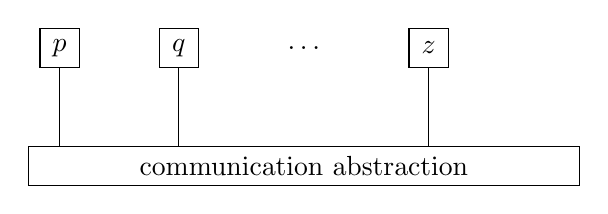
\begin{tikzpicture}
				\coordinate (start);
							
				%Nodes
				\node (rect) [draw,thin,minimum width=0.5cm,minimum height=0.5cm] (p) {$p$};
				\node (rect) [draw,thin,minimum width=0.5cm,minimum height=0.5cm, right=1cm of p] (q) {$q$};
				\node [right=1cm of q] (ldots) {$\ldots$};
				\node (rect) [draw,thin,minimum width=0.5cm,minimum height=0.5cm, right=1cm of ldots] (z) {$z$};
				
				\node (rect) [draw,thin,minimum width=7cm,minimum height=0.5cm, below=1.1cm of ldots] {communication abstraction};
				
				\node [below=1cm of p] (bp) {};
				\node [below=1cm of q] (bq) {};
				\node [below=1cm of z] (bz) {};
				
				%Lines
				\draw (p) -- (bp);
				\draw (q) -- (bq);
				\draw (z) -- (bz);
				
			\end{tikzpicture}
			\begin{enumerate}[-]
				\item Set of Processes $\Pi$ \\
				$\mid \Pi \mid = N$
				\item A process is an automaton
				\item A protocol is a set of processes
			\end{enumerate}
			\subsubsection{Execution}
			\begin{adjustwidth}{2em}{}
				\begin{enumerate}[-]
					\item Each computation step and every step of sending a message or receiving a message is an event
					\item An execution (history) is a sequence of all events of the processes as seen by a (hypothetical) global observer
					\item trace = execution
				\end{enumerate}
			\end{adjustwidth}
			\subsubsection{Properties}
			\begin{adjustwidth}{2em}{}
				Used for specifying the abstractions: \\
				\begin{enumerate}[\footnotesize{\textbullet}]
					\item \textbf{Safety properties} (\textit{something "bad" has not happened}) \\
					If a property $P$ has been violated in some execution $E$, then there exists a prefix $E'$ of $E$ such that in every extension of $E'$, property $P$ is violated
					\item \textbf{Liveness properties} (\textit{something "good" will happen in the future} [\textsc{eventually}]) \\
					Property $P$ can be satisfied by some extension $\stackrel{\sim}{E}$ of a given execution $E$
				\end{enumerate}
				\hfill \\
				\textit{Safety} or \textit{Liveness} alone is not very useful. Only combination of both properties.
			\end{adjustwidth}
			\subsubsection{Process Failures}
			\begin{adjustwidth}{2em}{}
				A process consists of different modules - if one of them fails the entire thing fails at once.
				\begin{enumerate}[-]
					\item[$\bigstar$] \underline{\textit{\textbf{Crashes}}}
					\item \textit{Omission failures }(\textit{message sending and receiving events are omitted})
					\item \textit{Crash-Recovery Failure}
					\begin{enumerate}[\tiny{\textbullet}]
						\item store(-) operation to write to stable storage
						\item upon recovery, one can restore(-) data from this stable storage
					\end{enumerate}
					\item \textit{Eavesdropping Fault}
					\item[$\bigstar$] \underline{\textit{\textbf{Arbitrary Fault (Byzantine Fault)}}}
				\end{enumerate}
			\end{adjustwidth}
		\end{adjustwidth}
		\subsection{Cryptographic Abstraction}
		\begin{adjustwidth}{2em}{2em}
			\begin{enumerate}[\footnotesize{\textbullet}]
				\item \textbf{\textit{Hash functions}} (SHA-256) \\
				$H:{ 0,1 } ^{\star} \rightarrow \{ 0,1 \} ^{k}$
				\begin{enumerate}[-]
					\item collision-free: difficult to find $x, x'$ with $x \neq x'$ and $H(x) = H(x')$
				\end{enumerate}
				\item \textbf{\textit{Message-Authentication-Code (MAC)}} (HMAC-SHA256)
				\begin{enumerate}[-]
					\item $\textit{authentication}(p, q, m) \rightarrow a$
					\item $\textit{verifyAuth}(p, q, m, a) \rightarrow$ \textsc{Yes/No}
				\end{enumerate}
				\item \textbf{\textit{Digital Signatures}} (RSA, (EC)DSA)
				\begin{enumerate}[-]
					\item $\textit{sign}(p, m) \rightarrow s$
					\item $\textit{verifySign}(p,m,s) \rightarrow$ \textsc{Yes/No}
					\item[$\bigstar$] \underline{\textit{Correctness}}: \\
					$\forall m,p: \ \textit{verifySign}(p, m, \textit{sign}(p,m)) \ =$ \textsc{Yes}
					\item[$\bigstar$] \underline{\textit{Security}}: \\
					$\forall m, p, s: \ \textit{verifySign}(p, m, s) \ =$ \textsc{No}, unless $p$ has executed $sign(p,m) \rightarrow s$
				\end{enumerate}
			\end{enumerate}
		\end{adjustwidth}
		\subsection{Communication Abstraction}
		\begin{adjustwidth}{2em}{2em}
			Every process can send messages to every other process.
			\subsubsection{Stubborn point-to-point links}
			\begin{adjustwidth}{2em}{}
				\textbf{\underline{Events:}}
				\begin{enumerate}[]
					\item $\langle sl.send \mid q,m \rangle$ \{ \textit{send message $m$ to process $q$}
					\item $\langle sl.deliver \mid p,m \rangle$ \{ deliver a received message $m$ from process $p$ 
				\end{enumerate}
				\textbf{\underline{Properties:}}
				\begin{enumerate}[]
					\item \underline{\textit{Stubborn delivery}:} \\
					If a process sends a message $m$ to process $q$, then $m$ is infinitely often delivered at $q$.
					\item \underline{\textit{No creation}:} \\
					If some process $q$ delivers some message $m$ from $p$ then process $p$ has previously sent $m$ to $q$.
				\end{enumerate}
			\end{adjustwidth}
			\subsubsection{Perfect point-to-point links}
			\begin{adjustwidth}{2em}{}
				\textbf{\underline{Events:}}
				\begin{enumerate}[]
					\item $\langle sl.send \mid q,m \rangle$
					\item $\langle sl.deliver \mid p,m \rangle$
				\end{enumerate}
				\textbf{\underline{Properties:}}
				\begin{enumerate}[]
					\item \underline{\textit{Reliable delivery}:} \\
					If a correct process sends a message $m$ to a correct process $q$ then $q$ eventually delivers $m$
					\item \underline{\textit{No creation}:} \\
					If process $q$ delivers some $m$ from process $p$ then $p$ has sent $m$ to $q$
					\item \underline{\textit{At-most-once delivery:}} \\
					Every message $m$ is delivered at most once from $p$ to $q$.
				\end{enumerate}
			\end{adjustwidth}
			\subsubsection{Alg. impl. perfect links (pl) from stubborn links (sl)}
			\begin{adjustwidth}{2em}{}
				\underline{\textsc{Init:}} \\
				$\mathbb{D} \leftarrow \emptyset$ \\
				\underline{upon} $\langle pl.send \mid q,m \rangle$ \underline{do}
				\begin{adjustwidth}{1em}{}
					trigger $\langle sl,send \mid q,m \rangle$ \\
					\underline{upon} $\langle sl.deliver \mid p,m \rangle$ \underline{do}
					\begin{adjustwidth}{1em}{}
						\underline{if} $(p,m) \not\in \mathbb{D}$ \underline{then}
						\begin{adjustwidth}{1em}{}
							$\mathbb{D} \leftarrow \mathbb{D} \cup \{ (p,m) \}$ \\
							trigger $\langle pl.deliver \mid p,m \rangle$ \\
							\ldots
						\end{adjustwidth}
					\end{adjustwidth}
				\end{adjustwidth}
			\end{adjustwidth}
		\end{adjustwidth}
		\subsection{Timing Assumptions}
		\begin{adjustwidth}{2em}{2em}
			\begin{enumerate}[\footnotesize{\textbullet}]
				\item \underline{\textbf{Asynchronous model} (\textit{Logical Timing})}
				\begin{enumerate}[-]
					\item \textbf{\textit{One Process}} \\
					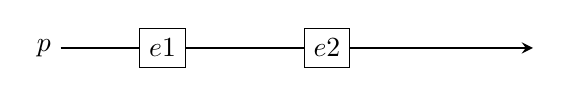
\begin{tikzpicture}
						%Nodes
						\node (rect) (p) {$p$};
						\node [right=6cm of p] (end) {};
					
						%Lines
						\draw[arrow] (p) -- (end);
					
						\node (rect) [draw,thin,fill=white,minimum width=0.5cm,minimum height=0.5cm, right=1cm of p] (e1) {$e1$};
						\node (rect) [draw,thin,fill=white,minimum width=0.5cm,minimum height=0.5cm, right=1.5cm of e1] (e2) {$e2$};
					\end{tikzpicture} \\
					If $e2$ happened after $e1$ in one process, we know the sequence of events.
					\item \textbf{\textit{Two Processes}} \\
					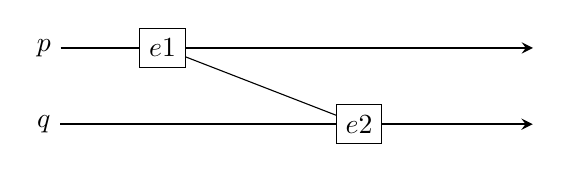
\begin{tikzpicture}
						%Nodes
						\node (rect) (p) {$p$};
						\node [right=6cm of p] (endp) {};
						
						\node (rect) [below=0.5cm of p] (q) {$q$};
						\node [right=6cm of q] (endq) {};
					
						%Lines
						\draw[arrow] (p) -- (endp);
						\draw[arrow] (q) -- (endq);
					
						\node (rect) [draw,thin,fill=white,minimum width=0.5cm,minimum height=0.5cm, right=1cm of p] (e1) {$e1$};
						\node (rect) [draw,thin,fill=white,minimum width=0.5cm,minimum height=0.5cm, right=3.5cm of q] (e2) {$e2$};
						
						\draw (e1) -- (e2);
					\end{tikzpicture} \\
					If we know that $e1$ caused $e2$, we know that $e2$ happened after $e1$.
					\item \textbf{\textit{Three processes}} \\
					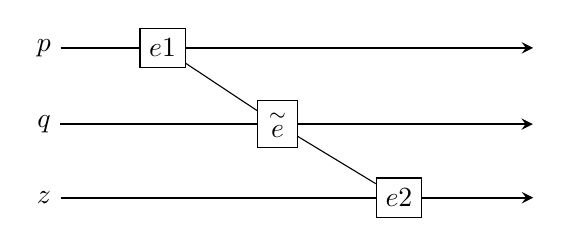
\begin{tikzpicture}
						%Nodes
						\node (rect) (p) {$p$};
						\node [right=6cm of p] (endp) {};
						
						\node (rect) [below=0.5cm of p] (q) {$q$};
						\node [right=6cm of q] (endq) {};
						
						\node (rect) [below=0.5cm of q] (z) {$z$};
						\node [right=6cm of z] (endz) {};
					
						%Lines
						\draw[arrow] (p) -- (endp);
						\draw[arrow] (q) -- (endq);
						\draw[arrow] (z) -- (endz);
					
						\node (rect) [draw,thin,fill=white,minimum width=0.5cm,minimum height=0.5cm, right=1cm of p] (e1) {$e1$};
						\node (rect) [draw,thin,fill=white,minimum width=0.5cm,minimum height=0.5cm, right=2.5cm of q] (et) {$\stackrel{\sim}{e}$};
						\node (rect) [draw,thin,fill=white,minimum width=0.5cm,minimum height=0.5cm, right=4cm of z] (e2) {$e2$};
						
						\draw (e1) -- (et);
						\draw (et) -- (e2);
					\end{tikzpicture} \\
					Transitivity holds across processes, so if $e1$ caused $\stackrel{\sim}{e}$ which cause $e2$, $e2$ happened after $e1$.
				\end{enumerate}
				\item Other time models exist
			\end{enumerate}
		\end{adjustwidth}
	\end{adjustwidth}
	
	\newpage
	
	\section{Timing Assumptions - March 3, 2020}
	\begin{adjustwidth}{2em}{2em}
		\subsection{Asynchronous System}
		\begin{adjustwidth}{2em}{2em}
			Logical clock creates a logical time
			\begin{enumerate}[-]
				\item Each process $p$ keeps a logical clock $lp$ (initially 0)
				\item When an event $e$ on $p$ occurs, then $lp \ \leftarrow \ lp + 1$
				\item When $p$ sends a message $m$ to $q$, then $p$ attaches a timestamp $ts(m) \ = \ lp$ to $m$
				\item When $p$ receives a message $m'$ with $ts(m')$, then $p$ sets $lp \ \leftarrow \ max\{lp, ts(m')\} + 1$
			\end{enumerate}
			\subsubsection{Happens-before relation}
			\begin{adjustwidth}{2em}{}
				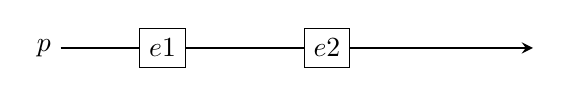
\begin{tikzpicture}
					%Nodes
					\node (rect) (p) {$p$};
					\node [right=6cm of p] (end) {};
					
					%Lines
					\draw[arrow] (p) -- (end);
					
					\node (rect) [draw,thin,fill=white,minimum width=0.5cm,minimum height=0.5cm, right=1cm of p] (e1) {$e1$};
					\node (rect) [draw,thin,fill=white,minimum width=0.5cm,minimum height=0.5cm, right=1.5cm of e1] (e2) {$e2$};
				\end{tikzpicture} \\
				\hfill \\
				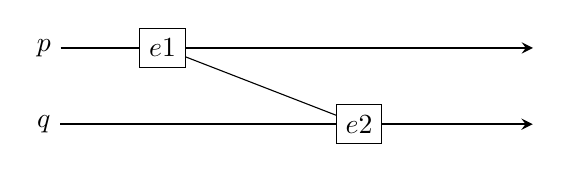
\begin{tikzpicture}
					%Nodes
					\node (rect) (p) {$p$};
					\node [right=6cm of p] (endp) {};
								
					\node (rect) [below=0.5cm of p] (q) {$q$};
					\node [right=6cm of q] (endq) {};
						
					%Lines
					\draw[arrow] (p) -- (endp);
					\draw[arrow] (q) -- (endq);
						
					\node (rect) [draw,thin,fill=white,minimum width=0.5cm,minimum height=0.5cm, right=1cm of p] (e1) {$e1$};
					\node (rect) [draw,thin,fill=white,minimum width=0.5cm,minimum height=0.5cm, right=3.5cm of q] (e2) {$e2$};
						
					\draw (e1) -- (e2);
				\end{tikzpicture} \\
				\hfill \\
				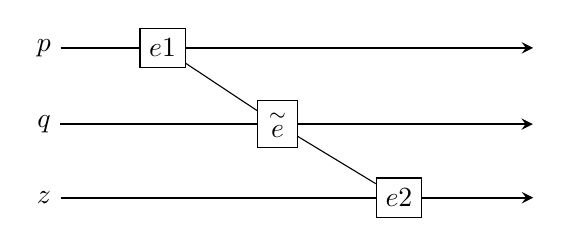
\begin{tikzpicture}
					%Nodes
					\node (rect) (p) {$p$};
					\node [right=6cm of p] (endp) {};
						
					\node (rect) [below=0.5cm of p] (q) {$q$};
					\node [right=6cm of q] (endq) {};
						
					\node (rect) [below=0.5cm of q] (z) {$z$};
					\node [right=6cm of z] (endz) {};
					
					%Lines
					\draw[arrow] (p) -- (endp);
					\draw[arrow] (q) -- (endq);
					\draw[arrow] (z) -- (endz);
					
					\node (rect) [draw,thin,fill=white,minimum width=0.5cm,minimum height=0.5cm, right=1cm of p] (e1) {$e1$};
					\node (rect) [draw,thin,fill=white,minimum width=0.5cm,minimum height=0.5cm, right=2.5cm of q] (et) {$\stackrel{\sim}{e}$};
					\node (rect) [draw,thin,fill=white,minimum width=0.5cm,minimum height=0.5cm, right=4cm of z] (e2) {$e2$};
						
					\draw (e1) -- (et);
					\draw (et) -- (e2);
				\end{tikzpicture} \\
				In each of these we can say that $e1$ happens before $e2$
			\end{adjustwidth}
			\subsubsection{Lemma}
			\begin{adjustwidth}{2em}{}
				$e1$ occurs at $p$ at $lp$ \\
				$e2$ occurs at $q$ at $lq$ \\
				$\Rightarrow$ $e1 \rightarrow e2$, then $lp \ < \ lq$, but not the other way round!
			\end{adjustwidth}
		\end{adjustwidth}
		\subsection{Synchronous System}
		\begin{adjustwidth}{2em}{2em}
			\underline{\textbf{\textsc{Either:}}} \\
			\begin{enumerate}[-]
				\item Assume every process has access to a real-time clock (\textit{\textbf{RTC}})
			\end{enumerate}
			\underline{\textbf{\textsc{Or:}}}
			\begin{enumerate}[-]
				\item Synchronous computation (bounds on computation time)
				\item Synchonous communication (bounds on message-transmission time)
			\end{enumerate}
			\textsc{\textbf{Careful!}} when synchrony, assumptions are needed for safety properties
		\end{adjustwidth}
		\subsection{Partially Synchronous Model}
		\begin{adjustwidth}{2em}{2em}
			\begin{enumerate}[-]
				\item Synchronous most of the time
				\item When asynchronous, must not violate safety
			\end{enumerate}
			Formally captured by abstraction of an eventually synchonous system.
			\begin{enumerate}[-]
				\item Initial period of asynchrony
				\item After some point in time (unknown to algorithm), system is synchonous
			\end{enumerate}
			\textsc{\textbf{Note:}} Abstract model will remain synchronous forever after sync-point. In practice, periods of synchrony and asynchrony alternate.
		\end{adjustwidth}
		\subsection{Abstracting Time}
		\begin{adjustwidth}{2em}{2em}
			\underline{\textbf{\textsc{Definition:}}} Perfect Failure Detecture $\mathbb{P}$ \\
			\underline{\textbf{\textsc{Event:}}} $\langle \mathbb{P}.\textit{Crash} \mid p \rangle$ denotes that process $p$ has crashed. \\
			\underline{\textbf{\textsc{Properties:}}}
			\begin{enumerate}[]
				\item \textsc{\textbf{Strong Completeness:}} \\
				\underline{Eventually} every process that has crashed is detected by all correct processes.
				\item \textsc{\textbf{Strong Accuracy:}} \\
				For any process $p$, if $p$ detects that $q$ crashed, then $q$ has crashed.
			\end{enumerate}
			\hfill \\
			\underline{Formally}, all processes are either alive \underline{forever} or they crash and stop. \\
			Suppose a notion of time in $\mathbb{N}$:
			\begin{enumerate}[]
				\item $C: \mathbb{N} \rightarrow \Pi$, $C(t)$ denotes the processes that are live at time $t$.
				\item $F: \mathbb{N} \rightarrow \Pi$, $F(t)$ denotes the proceses that are \underline{faulty} (crashed) at time $t$.
			\end{enumerate}
			$p \in F(t)$, then $\forall t' \geq t: \ p \in F(t')$ (crashes are irreversible)
			\begin{enumerate}[]
				\item $\mathbb{F} \ = \ \bigcup_{t \geq 0} F(t)$, set of all faulty processes
				\item $\mathbb{C} \ = \ \Pi \setminus \mathbb{F}$, set of all correct processes
			\end{enumerate}
			\begin{quote}
				\underline{Strong Completeness:} \\
				$\exists t: \forall p \in \mathbb{F}, \forall q \in \mathbb{C}: \exists t' \geq t: \langle \mathbb{P}.\textit{Crash} \mid p \rangle$ occurs on process $q$ at time $t'$. \\
				\underline{Strong Accuracy:} \\
				$\forall q \in \mathbb{C}$ if $\langle \mathbb{P}.\textit{Crash} \mid p \rangle$ occurs on process $q$ at time $t$ then $p \in F(t)$.
			\end{quote}
			\subsubsection{Implementing $\mathbb{P}$}
			\begin{adjustwidth}{2em}{}
				\begin{tabular}{lll}
					\begin{tabular}{l}
						\underline{Initialization:} \\
						\ \ start timer $\Delta$ \\
						\ \ alive $\leftarrow \Pi$ \\
						\ \ detected $\leftarrow \emptyset$ \\
						\\
						\underline{upon} timeout \underline{do}
						\ \ \underline{for all} $p \in \Pi$ \underline{do} \\
						\ \ \ \ \underline{if} $p \not\in \textit{alive} \wedge p \not\in \textit{detected}$ \underline{then}
						\ \ \ \ \ \ trigger $\langle \mathbb{P}.\textit{Crash} \mid p \rangle$ \\
						\ \ \ \ \ \ detected $\leftarrow$ detected $cup \{ p \}$ \\
						\ \ start timer with $\Delta$ \\
						\ \ alive $\leftarrow \emptyset$ \\
						\ \ send msg [\textsc{ping}] to all $p \in \Pi$ \\
						\hfill \\
						\underline{upon} receive msg. [\textsc{ping}] from $p$ \underline{do} \\
						\ \ send msg [\textsc{pong}] to $p$ \\
						\hfill \\
						\underline{upon} receiving [\textsc{pong}] from $p$ \underline{do} \\
						\ \ alive $\leftarrow$ alive $\cup \{ p \}$
					\end{tabular}
				\end{tabular}
			\end{adjustwidth}
			\hfill \\
			\hfill \\
			\underline{\textbf{\textsc{Definition:}}} Leader Election \\
			\underline{\textbf{\textsc{Event:}}} $\langle le.\textit{leader} \mid p \rangle$, elects $p$ to be leader \\
			\underline{\textbf{\textsc{Properties}} (Eventual Leadership):} \\
			Eventually, some process $l$ is elected leader by every correct process
			\begin{enumerate}[]
				\item \textbf{\textsc{Accuracy:}} \\
				If a process is elected leader then all previously elected leaders have crashed.
			\end{enumerate}
			\hfill \\
			\underline{\textbf{\textsc{Definition:}}} Eventually Perfect Failure Detector \\
			\underline{\textbf{\textsc{Events:}}} 
			\begin{enumerate}[]
				\item $\langle \diamond \mathbb{P}.\textit{Suspect} \mid p \rangle$, process $p$ is suspected.
				\item $\langle \diamond \mathbb{P}.\textit{Restore} \mid p \rangle$, process $p$ is thought to be alive.
			\end{enumerate}
			\underline{\textbf{\textsc{Properties}}}
			\begin{enumerate}[]
				\item \textbf{\textsc{Strong Completeness:}} \\
				Eventually, every process that has crashed is suspected by every correct process
				\item \textbf{\textsc{Eventual Strong Accuracy:}} \\
				Eventually, every process that has crashed is suspected permanently by every correct process.
			\end{enumerate}
			\hfill \\
			\begin{center}
				\begin{tabular}{|l|l|l|l|}
					\hline
					Model & Processes & Timing & \\
					\hline
					fail-stop & crash-stop & synchronous & $\langle \mathbb{P} \rangle$ \\
					fail-noisy & crash-stop & partially synchronous & $\langle \diamond\mathbb{P} \rangle$, $N > 2F$ \\
					fail-silent & crash-stop & asynchronous & $N > 2F$ \\
					\hline
				\end{tabular}
			\end{center}
		\end{adjustwidth}
	\end{adjustwidth}
	
	\newpage
	
	\section{System Models - March 11, 2020}
	\begin{adjustwidth}{-5em}{2em}
		\begin{tabular}{|l|l|l|l|l|}
			\hline
			\cellcolor{gray!80} CGR11 & \cellcolor{gray!80} processes & \cellcolor{gray!80} timing assumption & \cellcolor{gray!80} assumption & \cellcolor{gray!80} other names \\
			\hline
			fail-stop & crash & $\mathbb{P}$ & - & synchronous \\
			fail-noisy & crash & $\diamond \mathbb{P}, \Omega$ & $N > 2 \mathbb{F}$ & eventually synchronous \\
			fail-silent & crash & - & $N > 2 \mathbb{F}$ & asynchronous \\
			fail-silent randomized & crash & - & $N > 2 \mathbb{F}$, randomness & asynchronous randomized \\
			fail-revocery & crash-recovery & & & \\
			fail-arbitrary-noisy & fail-arbitrary & Byz. leader detector & $N > 3 \mathbb{F}$ & "BFT" (PBFT) \\
			fail-arbitrary-silent & -"- & - & $N > 3 \mathbb{F}$ & asynchronous Byzantine \\
			fail-arbitrary randomized & \textsc{Byzantine} & - & $N > 3 \mathbb{F}$ & randomized Byzantine fault model \\
			\hline
		\end{tabular}
	\end{adjustwidth}
	\begin{adjustwidth}{2em}{2em}
		\subsection{Chapter 3: Distributed Storage and Shared Memory}
		\begin{adjustwidth}{2em}{2em}
			\begin{enumerate}[-]
				\item Storage abstraction provided by distributed processes
				\item Here: simplified model where $\Pi = \mathbb{C}$, designated processes act as  writing/reading clients
			\end{enumerate}
			\subsubsection{Main Abstraction}
			\begin{adjustwidth}{2em}{}
				\underline{\textbf{\textit{Shared Read-/Write-Register}}}: \\
				\begin{tabular}{l}
					\underline{Operations:} \\
					\ \ read() $\rightarrow v$ \\
					\ \ write($v$) $\rightarrow$ ACK \\
					\\
					\underline{Sequential implementations:} \\
					\ \ \underline{state:} \\
					\ \ \ \ val, initially \textsc{null} \\
					\ \ \underline{function} read() \\
					\ \ \ \ return val \\
					\ \ \underline{function} write(v) \\
					\ \ \ \ val $\leftarrow$ v
					\ \ \ \ return ACK
				\end{tabular}
				\hfill \\
				\underline{\textbf{\textit{Module Register}}} (r): \\
				\begin{tabular}{l}
					\underline{Events:} \\
					\ \ $\langle r, \textsc{ Read} \rangle$ \\
					\ \ $\langle r, \textsc{ ReadResp} \mid v \rangle$ \\
					\ \ $\langle r, \textsc{ Write} \mid v \rangle$ \\\\
					\ \ $\langle r, \textsc{ WriteResp} \rangle$ (acknowledgement) \\
				\end{tabular}
				\hfill \\
				\underline{\textbf{\textit{Liveness:}}} \\
				every operation eventually returns a response \\
				\hfill \\
				\underline{\textbf{\textit{Safety:}}} \\
				Every read operation returns the value written by the "last write" operation, when no \underline{concurrent} operation. \\
				\hfill \\
				\underline{\textbf{\textit{Operations:}}} \\
				every operation modeled by two events
				\begin{enumerate}[-]
					\item Invocation event
					\item Completion event
				\end{enumerate}
			\end{adjustwidth}
			\subsubsection{Definition (Preceding)}
			\begin{adjustwidth}{2em}{}
				Operation $o_1$ \underline{precedes} operation $o_2$ if $o_1$ completes before $o_2$ is invoked.
			\end{adjustwidth}
			\subsubsection{Definition (Sequential)}
			\begin{adjustwidth}{2em}{}
				Operations $o_1$ and $o_2$ are \underline{sequential} if $o_1$ precedes $o_2$ or $o_2$ precedes $o_1$.
			\end{adjustwidth}
			\subsubsection{Definition (Concurrent)}
			\begin{adjustwidth}{2em}{}
				Operations $o_1$ and $o_2$ are \underline{concurrent} if they are not sequential.
			\end{adjustwidth}
			\subsubsection{Register Example}
			\begin{adjustwidth}{2em}{}
				\underline{\textbf{\textit{Register Domain}}}
				\begin{enumerate}[-]
					\item binary register $\{ 0,1 \}$
					\item multi-valued register
				\end{enumerate}
				\hfill \\
				\underline{\textbf{\textit{Register Types}}}
				\begin{enumerate}[-]
					\item (1,1) 1 writer, 1 reader (SRSW register (single-writer-single-reader))
					\item (1,N) 1 writer, N readers (MRSW register (multi-writer-single-reader))
					\item (N,N) N writers, N readers (MRMW register (multi-writer-multi-reader))
				\end{enumerate}
				\hfill \\
				\underline{\textbf{\textit{Semantics:}}}
				\begin{enumerate}[]
					\item \underline{\textbf{Safe:}} \\
					A read() not concurrent with a write returns the value written by the most recent write() operation (a safe register can return any object from the domain)
				\end{enumerate}
			\end{adjustwidth}
			\subsubsection{An unsafe register}
			\begin{adjustwidth}{2em}{2em}
				Implement a multi-valued register (mvr) from (many) binary registers. \\
				Domain $\mathbb{D} = [ 0,11 ]$ \\
				4 binary registers $br-0, br-1, br-2, br-3$ \\
				Notation mit function calls:
				\begin{enumerate}[]
					\item br-0.write(1)
					\item mvr.read()
				\end{enumerate}
				\hfill \\
				\begin{tabular}{|l|}
					\hline
					\cellcolor{gray!80} \underline{\textbf{\textit{MVR}}} \\
					\hline
					\ \ \underline{\textbf{state}} \\
					\ \ \ \ \textit{br-0, br-1, br-2, br-3} initially 0 \\
					\\
					\ \ \underline{\textbf{function}} mvr.write($v$) \\
					\ \ \ \ $(b_3b_2b_1b_0)_2\leftarrow v$ \\
					\ \ \ \ \underline{for} $i \leftarrow 0,...,3$ \underline{do} \\
					\ \ \ \ \ \ \textit{br-i}.write($b_i$) \\
					\ \ \ \ \textbf{return} \textsc{ACK} \\
					\\
					\ \ \underline{\textbf{function}} mvr.read() \\
					\ \ \ \ \underline{for} $i \leftarrow 0,...,3$ \underline{do} \\
					\ \ \ \ \ \ $v_i \leftarrow$ \textit{br-i}.read() \\
					\ \ \ \ \textbf{return} $(v_3v_2v_1v_0)_2z$ \\
					\hline
				\end{tabular}
				\hfill \\
				\hfill \\
				\underline{\textbf{\textit{Execution:}}} \textit{initially mvr stores 9 =} $(1001)_2$ \\
				\begin{center}
					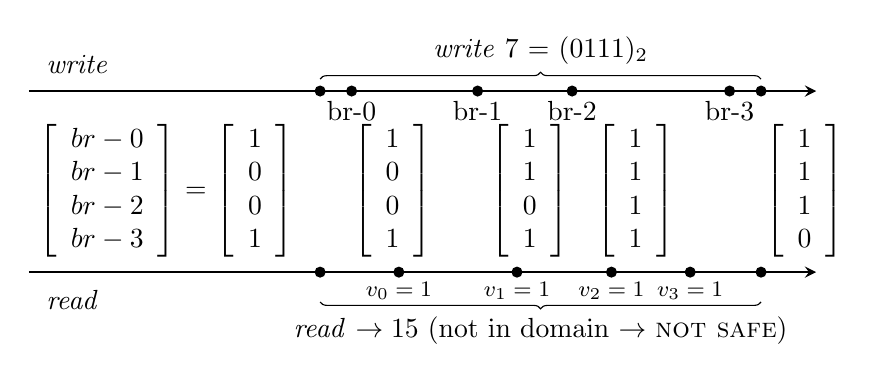
\begin{tikzpicture}[decoration=brace]
						%Coordinates
						\coordinate (startWrite);
						\coordinate [right=10cm of startWrite] (endWrite);
						\coordinate [below=2.3cm of startWrite] (startRead);
						\coordinate [right=10cm of startRead] (endRead);
						
						%Nodes
						\node [above right=0.1cm and 0.1cm of startWrite] {\textit{write}};
						\node [below right=0.1cm and 0.1cm of startRead] {\textit{read}};
						\node [below right=0.3cm and 0cm of startWrite] (1stEQ) {$\left[\begin{array}{c} br-0 \\ br-1 \\ br-2 \\ br-3\end{array}\right]$ = $\left[\begin{array}{c} 1 \\ 0 \\ 0 \\ 1\end{array}\right]$};
						\node [right=0.5cm of 1stEQ] (2ndEQ) {$\left[\begin{array}{c} 1 \\ 0 \\ 0 \\ 1\end{array}\right]$};
						\node [right=0.5cm of 2ndEQ] (3rdEQ) {$\left[\begin{array}{c} 1 \\ 1 \\ 0 \\ 1\end{array}\right]$};
						\node [right=0.1cm of 3rdEQ] (4thEQ) {$\left[\begin{array}{c} 1 \\ 1 \\ 1 \\ 1\end{array}\right]$};
						\node [right=0.9cm of 4thEQ] (5thEQ) {$\left[\begin{array}{c} 1 \\ 1 \\ 1 \\ 0\end{array}\right]$};
						
						%Circlets
						\fill (3.7,0) circle (2pt);
						\fill (4.1,0) circle (2pt) node[anchor=north] {br-0};
						\fill (5.7,0) circle (2pt) node[anchor=north] {br-1};
						\fill (6.9,0) circle (2pt) node[anchor=north] {br-2};
						\fill (8.9,0) circle (2pt) node[anchor=north] {br-3};
						\fill (9.3,0) circle (2pt);
						
						\fill (3.7,-2.3) circle (2pt);
						\fill (4.7,-2.3) circle (2pt) node[anchor=north] {\footnotesize{$v_0 = 1$}};
						\fill (6.2,-2.3) circle (2pt) node[anchor=north] {\footnotesize{$v_1 = 1$}};
						\fill (7.4,-2.3) circle (2pt) node[anchor=north] {\footnotesize{$v_2 = 1$}};
						\fill (8.4,-2.3) circle (2pt) node[anchor=north] {\footnotesize{$v_3 = 1$}};
						\fill (9.3,-2.3) circle (2pt);
						
						%Braces
						\draw[decorate, yshift=1ex] (3.7,0) -- node[above=0.4ex] {\textit{write} 7 = $(0111)_2$} (9.3,0);
						\draw[decorate, yshift=-2.5ex]  (9.3,-2.3) -- node[below=0.4ex] {\textit{read} $\rightarrow 15$ (not in domain $\rightarrow$ \textsc{not safe})} (3.7,-2.3);
											
						%Arrows
						\draw[arrow] (startWrite) -- (endWrite);
						\draw[arrow] (startRead) -- (endRead);
					\end{tikzpicture}
				\end{center}
				\hfill \\
				\underline{\textbf{\textit{Regular Semantics:}}}
				\begin{enumerate}[]
					\item Only single-writer registers
					\item \textit{Safety:}
					\begin{adjustwidth}{1em}{}
						\begin{enumerate}[]
							\item A read(), not concurrent with a write(), returns the most recently written value. \\
							Otherwise read() returns the most recently written value or the concurrently written values.
						\end{enumerate}
					\end{adjustwidth}
				\end{enumerate}
				\hfill \\
				\underline{\textbf{\textit{Atomic Semantics:}}} \textit{(assume values written are unique)}
				\begin{enumerate}[]
					\item \textit{Safety:}
					\begin{adjustwidth}{1em}{}
						\begin{enumerate}[(1)]
							\item -"-
							\item If read() $\rightarrow v$ and a subsequent read() $\rightarrow w$, then write($v$) preceds write ($w$) or write($v$) is concurrent to write($w$).
						\end{enumerate}
					\end{adjustwidth}
					\item \textit{Alternative characterization with linearizability}
					\begin{adjustwidth}{1em}{}
						\begin{enumerate}[]
							\item Collaps each operation to its linearization point, which must occur between invocation and response, and values returned satisfy the sequential specifications of the \underline{object}.
						\end{enumerate}
					\end{adjustwidth}
				\end{enumerate}
			\end{adjustwidth}
			\begin{adjustwidth}{-9em}{}
				\begin{center}
					\begin{tabular}{lll}
						\begin{tabular}{l}
							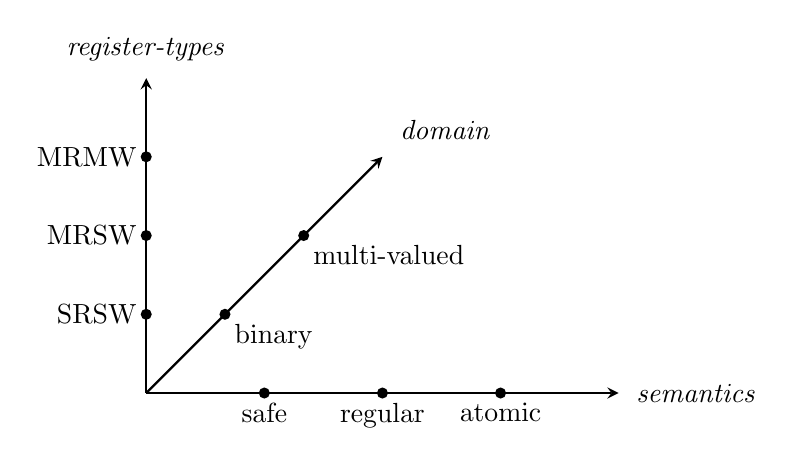
\begin{tikzpicture}
								%Coordinates
								\coordinate (origin);
								\coordinate [above=4cm of origin] (topY);
								\coordinate [right=6cm of origin] (topX);
								\coordinate [above right=3cm and 3cm of origin] (topZ);
								
								%Nodes
								\node [right=0.1cm of topX] (semantics) {\textit{semantics}};
								\node [above right=0.1cm and 0.1cm of topZ] (domain) {\textit{domain}};
								\node [above=0.1cm of topY] (registerTypes) {\textit{register-types}};
								
								\fill (0,1) circle (2pt) node[anchor=east]{SRSW};
								\fill (0,2) circle (2pt) node[anchor=east]{MRSW};
								\fill (0,3) circle (2pt) node[anchor=east]{MRMW};
								
								\fill (1.5,0) circle (2pt) node[anchor=north] {safe};
								\fill (3,0) circle (2pt) node[anchor=north] {regular};
								\fill (4.5,0) circle (2pt) node[anchor=north] {atomic};
								
								\fill (1,1) circle (2pt) node[anchor=north west] {binary};
								\fill (2,2) circle (2pt) node[anchor=north west] {multi-valued};
								
								
								%Lines
								\draw[arrow] (origin) -- (topX);
								\draw[arrow] (origin) -- (topY);
								\draw[arrow] (origin) -- (topZ);
								
							\end{tikzpicture}
						\end{tabular}
						&
						&
						\begin{tabular}{l}
							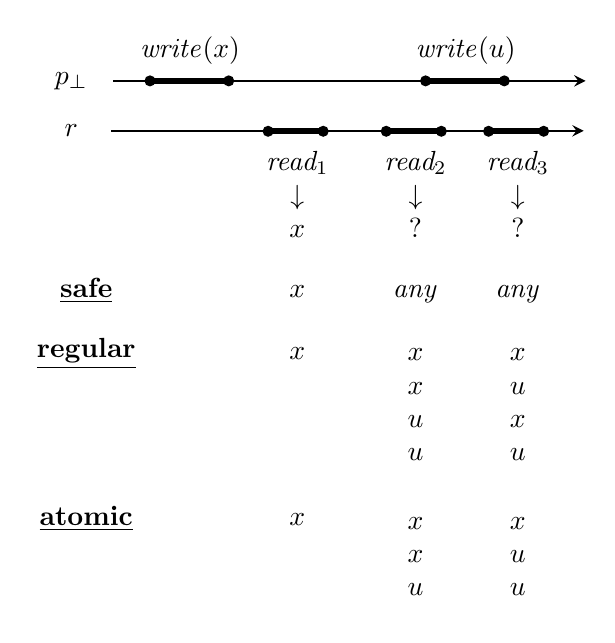
\begin{tikzpicture}
								%Nodes
								\node (pBot) {$p_{\bot}$};
								\node [below=0.2cm of pBot] (r) {$r$};
								
								%Coordinates
								\coordinate [right=0.2cm of pBot] (startWrite);
								\coordinate [right=0.3cm of r] (startRead);
								\coordinate [right=6cm of startWrite] (endWrite);
								\coordinate [right=6cm of startRead] (endRead);
								
								%Circlets
								\fill (1,0) circle (2pt);
								\fill (2,0) circle (2pt);
								\fill (4.5,0) circle (2pt);
								\fill (5.5,0) circle (2pt);
								\fill (2.5,-0.64) circle (2pt);
								\fill (3.2,-0.64) circle (2pt);
								\fill (4.0,-0.64) circle (2pt);
								\fill (4.7,-0.64) circle (2pt);
								\fill (5.3,-0.64) circle (2pt);
								\fill (6,-0.64) circle (2pt);
								
								%Arrows
								\draw[arrow] (startWrite) -- (endWrite);
								\draw[arrow] (startRead) -- (endRead);
								\draw[line width=0.8mm] (1,0) -- (2,0) node[above left=0.05cm and -0.3cm] {\textit{write}($x$)};
								\draw[line width=0.8mm] (4.5,0) -- (5.5,0) node[above left=0.05cm and -0.3cm] {\textit{write}($u$)};
								\draw[line width=0.8mm] (2.5,-0.64) -- (3.2,-0.64) node[below left=0.05cm and -0.4cm] (readOne) {$\begin{array}{c} \textit{read}_1 \\ \downarrow \\ x\end{array}$};
								\draw[line width=0.8mm] (4.0,-0.64) -- (4.7,-0.64) node[below left=0.05cm and -0.4cm] (readTwo) {$\begin{array}{c} \textit{read}_2 \\ \downarrow \\ ?\end{array}$};
								\draw[line width=0.8mm] (5.3,-0.64) -- (6,-0.64) node[below left=0.05cm and -0.4cm] (readThree) {$\begin{array}{c} \textit{read}_3 \\ \downarrow \\ ?\end{array}$};
								
								%TextNodes
								\node [below=0.2cm of readOne] (safeOne) {$x$};
								\node [left=2cm of safeOne] (safe) {\underline{\textbf{safe}}};
								\node [below=0.2cm of readTwo] (safeTwo) {\textit{any}};
								\node [below=0.2cm of readThree] (safeThree) {\textit{any}};
								
								\node [below=0.2cm of safe] (regular) {\underline{\textbf{regular}}};
								\node [below=0.4cm of safeOne] (regularOne) {$x$};								
								\node [below=0.2cm of safeTwo] (regularTwo) {$\begin{array}{c} x \\ x \\ u \\ u \end{array}$};
								\node [below=0.2cm of safeThree] (regularThree) {$\begin{array}{c} x \\ u \\ x \\ u \end{array}$};
								\node [below=1.5cm of regular] {\underline{\textbf{atomic}}};
								\node [below=1.7cm of regularOne] {$x$};								
								\node [below=0.2cm of regularTwo] {$\begin{array}{c} x \\ x \\ u \end{array}$};
								\node [below=0.2cm of regularThree] {$\begin{array}{c} x \\ u \\ u \end{array}$};
							\end{tikzpicture}
						\end{tabular}
					\end{tabular}
				\end{center}
			\end{adjustwidth}
			\subsubsection{Implementation of an (1,N) Regualar Register in Fail-Silent Mode}
			\begin{center}
				\begin{tabular}{|l|}
					\hline
					\cellcolor{gray!80} \underline{\textbf{\textit{Majority-Voting}}} \\
					\hline
					\underline{\textbf{state:}} \\
					\ \ \textit{val} \\
					\ \ \textit{ts} \\
					\ \ \textit{wts} $\leftarrow$ 0 //writer only \\
					\\
					\underline{\textbf{function}} rr.write($v$) \\ 
					\ \ $\textit{wts} \leftarrow \textit{wts + 1}$ \\
					\ \ \textit{send} message [\textsc{write}, $wts$, $v$] to all $p \in \Pi$ \\
					\ \ \underline{wait for} message [\textsc{write-ACK}] from $>N/2$ processors \\
					\ \ \underline{return} \textsc{ACK} \\											\\
					\underline{upon} \textit{receive} message [\textsc{write}, $ts'$, $v$] from $w$ \underline{do} \\
					\ \ $(val, ts) \leftarrow (v, ts')$ \\
					\ \ \textit{send} message [\textsc{write-ACK}] to $w$ \\
					\\
					\underline{upon} \textit{receive} message [\textsc{read}] from $r$ \underline{do} \\
					\ \ \textit{send} message [\textsc{readval}, $ts$, $val$] to $r$ \\
					\\
					\underline{\textbf{function}} rr.read() \\
					\ \ \textit{send} message [\textsc{read}] to all $p \in \Pi$ \\
					\ \ \underline{wait for} message [\textsc{readval}, $ts'$, $val'$] from $>N/2$ processors \\
					\ \ let $v$ be the value $val'$ among the received pairs with the highest timestamp \\
					\ \ \underline{return} $v$\\
					\\
					\hline
				\end{tabular}
			\end{center}
		\end{adjustwidth}
	\end{adjustwidth}
	
	\newpage
	
	\section{Implementations of Registers - March 18, 2020}
	\begin{adjustwidth}{2em}{2em}
		\subsection{\textsc{Regular} register implementation in \textit{fail-stop} model}
		\begin{adjustwidth}{2em}{2em}
			\begin{enumerate}[-]
				\item synchronous
				\item Perfect Failure Detector $\mathbb{P}$
			\end{enumerate} 
			\hfill \\
			\underline{\textbf{(1,N) regular register (\textit{onrr})}} \\
			tikz \\
			\begin{tabular}{l}
				\underline{Init:} \\
				\ \ $val \leftarrow 1$ \\
				\ \ $correct \leftarrow \Pi$ \\
				\\
				\underline{upon} $\langle \textit{onrr-Write} \mid v \rangle$ \underline{do} \\
				\ \ send message [\textsc{write}, v] to all $p \in \Pi$ //\textit{best-effort broadcast} \\
				\ \ \underline{wait for} receiving message [\textsc{ACK}] from all processes in \textit{correct} \\
				\ \ \underline{trigger} $\langle \textit{onrr-WriteResponse} \rangle$ \\
				\\
				\underline{upon} receive message [\textsc{write}, $v'$] from process $w$ \underline{do} \\
				\ \ $val \leftarrow v'$ \\
				\ \ send message [\textsc{ACK}] to $w$ \\
				\\
				\underline{upon} $\langle \mathbb{P}\textit{-Crash} \mid c \rangle$ \underline{do} \\
				\ \ \textit{correct} $\leftarrow$ \textit{correct $\setminus \{ c \}$ } \\
				\\
				\underline{upon} $\langle \textit{onrr-Read} \rangle$ \underline{do} \\
				\ \ \underline{trigger} $\langle \textit{onrr-ReadReturn} \mid \textit{val} \rangle$
			\end{tabular}
		\end{adjustwidth}
		\newpage
		\subsection{\textsc{Regular} register implementation in \textit{fail-silent} model}
		\begin{adjustwidth}{2em}{2em}
			\begin{enumerate}[-]
				\item asynchronous
			\end{enumerate} 
			\hfill \\
			\underline{\textbf{(1,N) regular register with $N > 2F$}} \\
			\begin{tabular}{l}
				\underline{Init:} \\
				\ \ $(ts, val) \leftarrow (o, \bot)$ \\
				\ \ $wts \leftarrow 0$ \\
				\ \ $rid \leftarrow 0$ \\
				\\
				\underline{upon} $\langle \textit{onrr-Write} \mid v \rangle$ \underline{do} \\
				\ \ $wts \leftarrow wts+1$ \\
				\ \ send message [\textsc{write}, $wts$, $v$] to all $p \in \Pi$ \\
				\ \ \underline{wait for} receiving message [\textsc{ACK}, $ts'$] s.t. $ts' = wts$ from $> \frac{N}{2}$ processes \\
				\ \ \underline{trigger} $\langle \textit{onrr-WriteResponse} \rangle$ \\
				\\
				\underline{upon} receive message [\textsc{write}, $ts'$, $v'$] from process $w$ \underline{do} \\
				\ \ \underline{if} $ts' > ts$ \underline{then} \\
				\ \ \ \ $(ts, val) \leftarrow (ts',v')$ \\
				\ \ send message [\textsc{ACK}, $ts'$] to $w$ \\
				\\
				\underline{upon} $\langle \textit{onrr-Read} \rangle$ \underline{do} \\
				\ \ $rid \leftarrow rid + 1$ \\
				\ \ send message [\textsc{READ}, $rid$] to all processes in $\Pi$ \\
				\ \ \underline{wait for} receive message [\textsc{VAL}, $r$, $ts'$, $v'$] s.t. $r = rid$ from $> \frac{N}{2}$ processes \\
				\ \ $\overline{v} \leftarrow$ value $v$ in the message with the highest timestamp $ts'$ \\
				\ \ \underline{trigger} $\langle onrr-\textit{ReadReturn} \mid \overline{v} \rangle$ \\
				\\
				\underline{upon} receiving message [\textsc{Read}, $r$] from process $p$ \underline{do} \\
				\ \ send message [\textsc{VAL}, $r$, ts, val] to $p$
			\end{tabular}
		\end{adjustwidth}
		\subsection{Example execution}
		\begin{adjustwidth}{2em}{2em}
			tikz
		\end{adjustwidth}
		\newpage
		\subsection{Make Algorithm (\textsc{above}) (Alg. 4.2) \textsc{atomic}}
		\begin{adjustwidth}{2em}{2em}
			(1,N)-\textsc{atomic} register (\textit{onar}) \\
			\hfill \\
			\begin{tabular}{l}
				\underline{upon} $\langle onar-\textit{Read} \rangle$ \underline{do} \\
				\ \ $rid \leftarrow rid + 1$ \\
				\ \ send message [\textsc{READ}, $rid$] to all processes in $\Pi$ \\
				\ \ \underline{wait for} receive message [\textsc{VAL}, $r$, $ts'$, $v'$] s.t. $r = rid$ from $> \frac{N}{2}$ processes \\
				\ \ $(rts, rval) \leftarrow ts',v'$-pair from \textsc{VAL} message with highest $ts'$ \\
				\ \ send message [\textsc{RWRITE}, $rts$, $rval$] to all $p \in \Pi$ \\
				\ \ \underline{wait for} receiving message [\textsc{RACK}, $rts'$] s.t. $rts' = rts$ from $> \frac{N}{2}$ processes \\
				\ \ \underline{trigger} $\langle \textit{onrr-ReadResponse} \mid rval \rangle$ \\
				\\
				\underline{upon} receive message [\textsc{RWRITE}, $ts'$, $val'$ from $r$ \underline{do} \\
				\ \ \underline{if} $ts' > ts$ \underline{then} \\
				\ \ \ \ $(ts, val) \leftarrow (ts',v')$ \\
				\ \ send message [\textsc{RACK}, $ts'$] to $r$ \\
			\end{tabular}
			\hfill \\ \\
			\underline{\textbf{start:}} (1,N) \textsc{regular} register \\
			\underline{\textbf{intermediate:}} (1,1) \textsc{atomic} register \\
			\underline{\textbf{goal:}} (1,N) \textsc{atomic} register \\
		\end{adjustwidth}
		\subsection{From (1,1) \textsc{atomic} to (1,N) \textsc{atomic} register}
		\begin{adjustwidth}{2em}{2em}
			tikz \\
			\hfill \\
			\underline{\textbf{Transformation:}} \\
			\textit{implements:} (1,N) \textsc{atomic} register (\textit{onar}) \\
			\textit{uses:} (1,1) \textsc{atomic} register ($u^2 :$ \textit{ooar.i.j}) \\
			\begin{tabular}{l}
				\underline{Init:}
				\ \ $ts \leftarrow 0$ \\
				\\
				\underline{operation} \textit{onar-}\textsc{Write}($v$) \underline{is} \\
				\ \ $ts \leftarrow ts + 1$ \\
				\ \ \underline{for} $p \in \Pi$ \underline{do} \\
				\ \ \ \ \textit{ooar.p.w}-\textsc{Write}(($ts,v$)) \\
				\ \ \textbf{return} \textsc{ACK} \\
				\\
				\underline{operation} \textit{onar-}\textsc{Read}() \underline{is} \\
				\ \ readList $\leftarrow []$ \\
				\ \ \underline{for} $p \in \Pi$ \underline{do} \\
				\ \ \ \ readList[p] $\leftarrow$ ooar.self.p-\textsc{Read}() \\
				\ \ (maxts, maxval) $\leftarrow$ highest(readList) \\
				\ \ \underline{for} $p \in \Pi$ \underline{do} \\
				\ \ \ \ ooar.p.self-\textsc{Write}((maxts, maxval)) \\
				\ \ \textbf{return} maxval
			\end{tabular}
		\end{adjustwidth}
		\subsection{From (1,N) \textsc{atomic} to (N,N) \textsc{atomic} register}
		\begin{adjustwidth}{2em}{2em}
			tikz \\
			\hfill \\
			\begin{enumerate}[-]
				\item writer uses highest timestamp that it reads
				\item timestamps become $(ts, \textit{index})$ duples (index of process)
			\end{enumerate}
		\end{adjustwidth}
		\subsection{Register Implementation in \textsc{Byzantine} Model ($N > 3F$)}
		\begin{adjustwidth}{2em}{2em}
			tikz01 \\
			tikz02 \\
			\begin{enumerate}[-]
				\item relax the specification
				\item introduce data authentication using digital signature
			\end{enumerate}
		\end{adjustwidth}
	\end{adjustwidth}
	
	\newpage
	
	\section{Byzantine Distributed Storage - March 25, 2020}
	\begin{adjustwidth}{2em}{2em}
		\subsection{Specification}
		\begin{adjustwidth}{2em}{2em}
			tikz \\
			\subsubsection{$(1,N)$-\textsc{regular} Register}
			\begin{adjustwidth}{2em}{}
				\textsc{in:} $\langle \textit{Read} \rangle$ \hspace{1.2cm} \textsc{out:} $\langle \textit{ReadReturn} \mid v \rangle$ \\
				\textsc{in:} $\langle \textit{Wirte} \mid v \rangle$ \hspace{1cm}\textsc{out:} $\langle WriteReturn \rangle$ \\
				\begin{enumerate}[-]
					\item \textbf{Termination:} \\
					Every operation eventually terminates
					\item \textbf{Validity:} \\
					every \textit{read} returns either \underline{the} concurrently written value or the most recently written value
				\end{enumerate}
				\begin{center}
					\begin{tabular}{l}
						\underline{Init:} \\
						\ \ $(ts, val, sig) \leftarrow (\bot , \bot , \bot)$ \\
						\ \ $wts \leftarrow 0$ \\
						\\
						\underline{upon} \textit{write}($v$) \underline{do} \\
						\ \ $wts \leftarrow wts + 1$ \\
						\ \ $\sigma \leftarrow \textit{sign}(\textsc{write} \| wts \| v)$ \\
						\ \ send message [\textsc{write}, $wts$, $v$, $\sigma$]  to all processes \\
						\ \ \underline{wait for} messages [\textsc{ACK}, $ts'$] s.t. $ts'=wts$ from $> \frac{n+f}{2}$ processes (\textsc{Byzantine} quorum) \\
						\\
						\underline{upon} receive message [\textsc{write}, $ts'$, $v'$, $\sigma '$] \underline{do} \\
						\ \ \underline{if} $ts' > ts$ \underline{then} \\
						\ \ \ \ $(ts, val, \sigma) \leftarrow (ts', v', \sigma ')$ \\
						\ \ send message [\textsc{ACK}, $ts'$] to writer $w$ \\
						\\
						\underline{upon} \textit{read()} \underline{do} \\
						\ \ send message [\textsc{read}] to all processes \\
						\ \ \underline{wait for} message [\textsc{value}, $ts'$, $v'$, $\sigma '$] from $> \frac{n+f}{2}$ with \textit{verifySign}($\sigma'$, \textsc{write} $\| ts' \| v'$) = \textsc{true} \\
						\ \ let $v$ be the received value $v'$ from message with the highest timestamp $ts'$ \\
						\ \ \textbf{return} $v$ \\
						\\
						\underline{upon} [\textsc{read}] \ldots					
					\end{tabular}
				\end{center}
				\newpage
				\begin{enumerate}[-]
					\item \textbf{Termination} \\
					$n$ replicas and $f$ faulty $\Rightarrow$ $\geq n-f$ responses \\
					\underline{Show:} $n-f > \frac{n+f}{2}$, if $n > 3f$\\
					\[
						n-f > \frac{n+f}{2} \textit{, if } n > 3f \ldots
					\]
					\item \textbf{Validity:} \\
					tikz
					\item \textbf{Safety:} \\
					$Q_w$ quorum used by writer \\
					$Q_r$ quorum used by reader \\
					$\mid Q_w \mid > \frac{n+f}{2}$ \\
					$\mid Q_r \mid > \frac{n+f}{2}$ \\
					\underline{Show:} There exists at least one correct process in $Q_w \cap Q_r$ \
					Suppose not: \\
					Count number of distinct correct processes in $Q_w \cap Q_r$ \\
					number is $\geq \mid Q_w \mid - f + \mid Q_r \mid - f > \frac{n+f}{2} - f + \frac{n-f}{2} - f = n - f$ \\
					$\Rightarrow$ So there exists at least one correct process in $Q_w \cap Q_r$
				\end{enumerate}
			\end{adjustwidth}
			\subsubsection{Can we implement this w/o signatures?}
			\begin{adjustwidth}{2em}{}
				tikz \\
				\begin{enumerate}[-]
					\item could return $c$ default value
					\item this idea can be turned into for emulating < \underline{safe} \textsc{Byzantine} registers assuming $n > 4f$ processes
					\item (2-round protocol with $n > 3f$ exists...)
				\end{enumerate}
			\end{adjustwidth}
			\subsubsection{Practical Leaderless Replication}
			\begin{adjustwidth}{2em}{}
				\begin{enumerate}[-]
					\item clients send request directly to replicas
					\item possibly via some coordinator
					\item tikz
					\item Consistency of the stored data
					\begin{enumerate}[\small{\textbullet}]
						\item auxiliaty service within storage system will eliminate differences - "\textit{anti-entropy}"
						\item \textit{read-repair} by reading clients that detect inconsistent clients
					\end{enumerate}
					\item Quorums for reading and writing \\
					$r$ - replicas for reading \\
					$w$ - replicas for writing \\
					so far: r = w $> \frac{n}{2}$ \\
					$r = 1, w = n$ read-one write-all \\
					$r = n, w = 1$ read-all write-one
					\item \textbf{Strong Consistency} iff $r+w>n$ \\
					Some systems use $r+w \leq n$
				\end{enumerate}
			\end{adjustwidth}
		\end{adjustwidth}
		\subsection{Key-Value Store (KVS)}
		\begin{adjustwidth}{2em}{2em}
			tikz \\
			\begin{enumerate}[-]
				\item Replica set usually differs for each pair
				\item Semantics is not formally specified
				\begin{enumerate}[\ldots]
					\item too expensive
					\item atomic problematic because the reader would write
				\end{enumerate}
				\item Conflicts?
				\begin{enumerate}[\small{\textbullet}]
					\item resolved using heuristic methods
					\item last-write wins policy
					\begin{enumerate}[\ldots]
						\item data loss is possible
					\end{enumerate}
				\end{enumerate}
				\item Practical system ensure usually a notion of \underline{eventual consistency}
				\item Some systems let clients merge conflicting written values
				\begin{enumerate}[\small{\textbullet}]
					\item often easy for applications
					\item very difficult in general
					\item[\ldots] \textsc{Amazon} Dynamo \\
					tikz
				\end{enumerate}
			\end{enumerate}
		\end{adjustwidth}
	\end{adjustwidth}
	
	\newpage
	
	\section{\textsc{Chapter} 4: Reliable Broadcast - April 01, 2020}
	\begin{adjustwidth}{2em}{2em}
		\subsection{Definition}
		\begin{adjustwidth}{2em}{2em}
			(\textsc{in}) $\langle \textsc{Broadcast} \mid m \rangle$ "\textit{broadcast a message} $m$" \\
			(\textsc{out}) $\langle \textsc{Deliver} \mid p, m \rangle$ "\textit{delivers a message} $m$ \textit{from sender} $p$" \\
			\begin{center}
				tikz
			\end{center}
		\end{adjustwidth}
		\subsection{Best-Effort Broadcast (\textsc{Unreliable})}
		\begin{adjustwidth}{2em}{2em}
			\subsubsection{Definition (\textsc{Validity}):}
			\begin{adjustwidth}{2em}{}
				If a \textit{correct} process broadcasts a message $m$, then every \textit{correct} process eventuall delivers $m$.
			\end{adjustwidth}
			\subsubsection{Definition (\textsc{No Duplication}):}
			\begin{adjustwidth}{2em}{}
				No message is delivered more than once.
			\end{adjustwidth}
			\subsubsection{Definition (\textsc{No Creation}):}
			\begin{adjustwidth}{2em}{}
				If a process delivers a message $m$ with sender $s$, then $m$ was previously broadcasted by process $s$.
			\end{adjustwidth}
		\end{adjustwidth}
		\subsection{Messages are \textsc{unique}}
		\begin{adjustwidth}{2em}{2em}
			\textit{How do we ensure this in practice?}
			.
			.
			.
		\end{adjustwidth}
		\subsection{Reliable Broadcast}
		\begin{adjustwidth}{2em}{2em}
			\subsubsection{Definition:}
			\begin{adjustwidth}{2em}{}
				Same properties as (unreliable) best-effort broadcast.
				\paragraph{Agreement:}
				\begin{adjustwidth}{1em}{}
					If a message $m$ is delivered by a \textit{correct} process then every \textit{correct} process eventually delivers $m$. \\
					\begin{center}
						tikz
					\end{center}
				\end{adjustwidth}
			\end{adjustwidth}
		\end{adjustwidth}
		\subsection{\textsc{Eager} Reliable Broadcast}
		\begin{center}
			\begin{tabular}{l}
				\underline{Init:}
				\ \ \textit{delivered} $\leftarrow \emptyset$ \\
				\\
				\underline{upon} $\langle \textit{rb-}\textsc{Broadcast} \mid m \rangle$ \underline{do} \\
				\ \ send message [\textsc{Data}, \textit{self}, $m$] to all $p \in \Pi$ \\
				\\
				\underline{upon} receive message [\textsc{Data}, $s$, $m$] from $q$ \underline{do} \\
				\ \ \underline{if} $m \not\in \textit{delivered}$ \underline{then} \\
				\ \ \ \ \textit{delivered} $\cup \leftarrow \{ m \}$ \\
				\ \ \ \ send message [\textsc{Data}, $s$, $m$] to all $p \in \Pi$ \\
				\ \ \ \ trigger $\langle \textit{rb-}\textsc{Deliver} \mid s, m \rangle$
			\end{tabular}
		\end{center}
		\begin{adjustwidth}{2em}{2em}
			\subsubsection{Implementation:}
			\begin{center}
				tikz
			\end{center}
			\begin{adjustwidth}{2em}{}
				\textbf{A process that crashes:} \\
				All modules crash simultaneously.
			\end{adjustwidth}
			\subsubsection{How adequate is this (basic) reliable broadcast?}
			\begin{center}
				tikz
			\end{center}
			\begin{adjustwidth}{2em}{}
			\end{adjustwidth}
		\end{adjustwidth}
		\subsection{\textsc{Uniform} Reliable Broadcast}
		\begin{adjustwidth}{2em}{2em}
			\subsubsection{Definition:}
			\begin{adjustwidth}{2em}{}
				Same properties as regular reliable broadcast.
				\paragraph{Uniform Agreement:}
				\begin{adjustwidth}{1em}{}
					If a process delivers a message $m$, then every correct process eventually delivers $m$.
					\begin{center}
						tikz
					\end{center}
				\end{adjustwidth}
			\end{adjustwidth}
			\subsubsection{Implementation of URB in async. netw. with $f$ crashes and $N > 2f$}					
			\begin{center}
				\begin{tabular}{l}
					$\textit{pending} \leftarrow \emptyset$ \\
					$ack[] \leftarrow []$ \\
					$\textit{delivered} \leftarrow \emptyset$
					\\
					\underline{upon} $\langle \textit{urb-}\textsc{Broadcast} \mid m \rangle$ \underline{do} \\
					\ \ \textit{pending} $\cup \leftarrow \{ (\textit{self}, m) \}$ \\
					\ \ send message [\textsc{Data}, \textit{self}, $m$] to all $p \in \Pi$ \\
					\\
					\underline{upon} receive message [\textsc{Data}, $s$, $m$] from $q$ \underline{do} \\
					\ \ $ack[m] \leftarrow ack[m] \cup \{ q \}$ \\
					\ \ \underline{if} ($s,m$) $\not\in$ \textit{pending} \underline{then} \\
					\ \ \ \ \textit{pending} $\leftarrow \{ (s,m) \}$ \\
					\ \ \ \ send message [\textsc{Data}, $s$, $m$] to all $p \in \Pi$ \\
					\\
					\underline{upon} $\exists(s,m) \in \textit{pending} \&\& m \not\in \textit{delivered}$ s.t. $\mid ack[m] \mid \ > \frac{N}{2}$ \underline{do} \\
					\ \ \textit{delivered} $\cup\leftarrow \{ m \}$ \\
					\ \ trigger $\langle \textit{urb-}\textsc{Deliver} \mid s,m \rangle$
				\end{tabular}
				\hfill \\
				tikz
			\end{center}
			\begin{adjustwidth}{2em}{}
				\begin{enumerate}[\small{\textbullet}]
					\item If $q$ delivers $m$, then it has received the \textsc{Data} messages from $> \frac{N}{2}$ processes
					\item Since $f < \frac{n}{2}$, at least one \textsc{Data} message was sent by a correct process, this process has sent $m$ ro all other processes
					\item All correct processes eventually send \textsc{Data} message containing $m$
					\item all correct processes eventually deliver $m$
				\end{enumerate}
			\end{adjustwidth}
		\end{adjustwidth}
		\subsection{Order}
		\begin{center}
			tikz
		\end{center}
		\begin{adjustwidth}{2em}{2em}
			\subsubsection{\textsc{FIFO}-Order Broadcast}
			\begin{adjustwidth}{2em}{}
				per-sender order
				\paragraph{Interface}
				\begin{adjustwidth}{1em}{}
					Same as reliable broadcast
				\end{adjustwidth}
				\paragraph{Properties}
				\begin{adjustwidth}{1em}{}
					\begin{enumerate}[-]
						\item Validity
						\item No Duplication
						\item No creation
						\item Agreement
						\item FIFO-Order (\textbf{if} bc. $m_1 \rightarrow m_2$ \textbf{then} del. $m_1 \rightarrow m_2$) \\
						If process broadcasts $m_1$ and subsequently broadcasts $m_2$, then no process delivers $m_2$ unless it has also delivered $m_1$ before.
					\end{enumerate}
				\end{adjustwidth}
				\paragraph{Implementation}
				\begin{adjustwidth}{1em}{}
					\begin{enumerate}[\small{\textbullet}]
						\item Each process adds a (local) sequence number to every payload message
						\item For each sender, every receiver delivers payload messages according to the sequence number (requiring buffering)
					\end{enumerate}
				\end{adjustwidth}
			\end{adjustwidth}
			\subsubsection{Causal Order (broadcast):}
			\begin{center}
				tikz
			\end{center}
			\begin{adjustwidth}{2em}{}
				\textbf{Prevent such violations of causal order:}
				\begin{enumerate}[-]
					\item keep track of complete history of past delivered messages
					\item Keep a counter messages for wach sender \\
					\begin{center}
						tikz
					\end{center}
				\end{enumerate}
			\end{adjustwidth}
		\end{adjustwidth}
	\end{adjustwidth}
	
	\newpage
	
	\section{8th Lecture - \today}
	\begin{adjustwidth}{2em}{2em}
		\subsection{sub}
		\begin{adjustwidth}{2em}{2em}
			\subsubsection{subsub}
			\begin{adjustwidth}{2em}{}
			\end{adjustwidth}
		\end{adjustwidth}
	\end{adjustwidth}
\end{document}